\section{Einleitung}
Ziel dieses Versuchs ist es den RLC-Schwingkreis zu untersuchen.
\section{Theorie}
\label{sec:Theorie}
\subsection{Die gedämpfte Schwingung des RLC-Schwingkreises}
Der in Abbildung \ref{fig:rlc} gezeigte Schaltkreis besteht aus einer Spule, einem Kondensator und einem ohmschen Wiederstand.
Der Kondensator und die Spule sind speicherfähige Bauteile.
Dies bedeutet, dass beide Bauteile als Energiespeicher fungieren.
\begin{figure}[H]
    \centering
    \caption{RLC-Schwingkreis.\cite{v354}}
    \label{fig:rlc}
    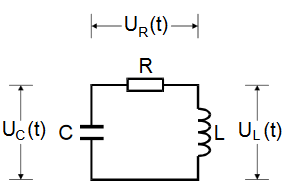
\includegraphics[width=\textwidth-20em]{content/RLCKreis.png}
\end{figure}
\noindent
Wird dem System elektrische Energie zugeführt, so kann diese zwischen den beiden Bauteilen oszillieren.
Der Widerstand wandelt die elektrische Energie in Wärme um.
Die Amplitude der Schwingung nimmt ab, sie ist gedämpft.
Mit der zweiten Kirchhoffschen Regel lässt sich die Gleichung für das vorliegende System aufstellen.
Es folgt:
\begin{equation}
  U_R(t)+U_C(t)+U_L(t) = 0
\end{equation}
oder anders
\begin{equation}
  \label{eq:gl1}
  L\frac{dI}{dt}+RI+\frac{Q}{C}=0 .
\end{equation}
Unter einbezug von
\begin{equation}
  I = \frac{dQ}{dt} ,
\end{equation}
folgt für Gleichung\eqref{eq:gl1}:
\begin{equation}
  \label{eq:gl2}
  \frac{d^2I}{dt^2}+\frac{R}{L}\frac{dI}{dt}+\frac{1}{LC}I =0
\end{equation}
 Die so erhaltene Differentialgleichung lässt sich über den Ansatz
 \begin{equation}
   \label{eq:gl3}
   I(t) = A e^{i\omega t}
 \end{equation}
lösen.
Die Konstante $\omega$ muss demnach einen der folgenden Werte annehmen:
\begin{equation}
  \omega_\text{1,2} = i \frac{R}{2L} \pm \sqrt{\frac{1}{LC} - \frac{R^2}{4L^2}}
\end{equation}
Somit ist die Lösung der Dgl. :
\begin{equation}
  I(t) = A_1 e^{i \omega t} + A_2 e^{i \omega t}
\end{equation}
Zweckmäßig werden die Abkürzungen
\begin{equation*}
  2\pi \mu := \frac{R}{2L}
\end{equation*}
und
\begin{equation*}
  2 \pi \upsilon = \sqrt{\frac{1}{LC}-\frac{R^2}{4L^2}}
\end{equation*}
eingeführt.
Die Lösung lässt ich dann in der Form
\begin{equation}
\label{eq:steig}
  I(t)= e^{-  2\pi \mu t} (A_1 e^{2 i \pi \upsilon t} + A_2 e^{-2 i \pi \upsilon t})
\end{equation}
schreiben.
Die Gestalt von $I(t)$ hängt davon ab ob $\frac{1}{LC}$ größer oder kleiner als $\frac{R^2}{4L^2}$ ist.
Der erste Fall ist, dass $\frac{1}{LC}<\frac{R^2}{4L^2}$.
Dann ist $I(t)$ reel, wodurch $A_1=A_2$ sein muss.
Durch den Ansatz
\begin{equation}
  A_1 = \frac{1}{2}A_0 e^{i \eta}
\end{equation}
und
\begin{equation}
A_2 = \frac{1}{2}A_0 e^{-i \eta}
\end{equation}
folgt die Lösung der gedämpften Schwingung:
\begin{equation}
  I(t) = A_0 e^{- 2 \pi \mu t} \cos(2 \pi \upsilon t + \eta)
\end{equation}
Die Schwingungsdauer besitzt den Wert:
\begin{equation}
  T = \frac{1}{\upsilon}=\frac{2 \pi}{\sqrt{\frac{1}{LC}-\frac{R^2}{4L^2}}}
\end{equation}
Die Abkligsdauer, welche angibt nach welcher Zeit die Amplitude um den e-ten Teil ihres ursprünglichen Wertes abgenommen hat, ergibt sich zu:
\begin{equation}
  T_\text{ex}=\frac{1}{2 \pi \mu}=\frac{2L}{R}
\end{equation}
In Abbildung \ref{fig:daempf} ist die Gestalt der gedämpften Schwingun zu sehen.
\begin{figure}[H]
    \centering
    \caption{Darstellung einer gedämpften Schwingung mit einhüllender.\cite{v354}}
    \label{fig:daempf}
    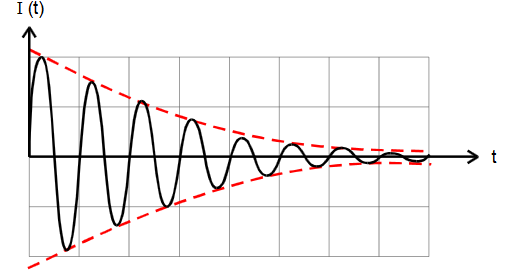
\includegraphics[width=\textwidth-20em]{content/daempfung.png}
\end{figure}
\noindent
Der zweite Fall tritt ein, wenn $\frac{1}{LC}<\frac{R^2}{4L^2}$ ist.
Die Lösung $I(t)$ hat dann keinen oszillatorischen Anteil mehr.
Es liegt also ein Relaxationsverhalten vor.
$I(t)$ kann entweder einen Grenzwert erreichen oder sofort monoton gegen Null gehen.
Hervorzuheben ist der Spezialfall des aperiodischen Grenzfalls.
Dann ist $\frac{1}{LC}=\frac{R^2}{4L^2}$ also $\upsilon=0$, womit folgt:
\begin{equation}
  I(t)=Ae^{-\frac{R}{2L}t}=Ae^{-\frac{t}{\sqrt{LC}}}
\end{equation}
Hier geht die Stromstärke(ohne Nulldurchlauf) am schnellsten gegen Null.
In Abbildung \ref{fig:ap} werden die möglichen Verläufe bei aperiodischer Dämpfung skizziert.
\begin{figure}[H]
    \centering
    \caption{Mögliche Zeitverläufe des Stroms bei aperiodischer Dämpfung.\cite{v354}}
    \label{fig:ap}
    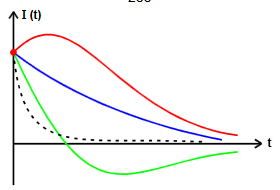
\includegraphics[width=\textwidth-20em]{content/apgrenz.png}
\end{figure}
\noindent
\subsection{Die erzwungene Schwingung}
An den gedämpften Schwingkreis wird eine Spannungsquelle angeschlossen, welche eine sinusförmige Spannung der Form

\begin{equation*}
  U(t)= U_0 e^{i\omega t}
\end{equation*}
liefert.
Dieser Aufbau wird in Abbildung \ref{fig:erzw} skizziert.
\begin{figure}[H]
    \centering
    \caption{RLC-Schwingkreis mit harmonischer Anregung.\cite{v354}}
    \label{fig:erzw}
    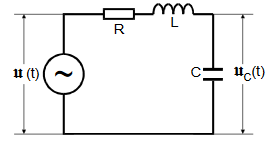
\includegraphics[width=\textwidth-20em]{content/erzwungen.png}
\end{figure}
\noindent
Analog zur Gleichung\eqref{eq:gl2} folgt:
\begin{equation}
  LC\frac{d^2 U_c}{dt^2} +RC \frac{d U_c}{dt}+U_c = U_0 e^{i\omega t}
\end{equation}
Es soll nun betrachtet werden wie die Amplitude $U_c$ der Kondesatorspannung und ihr Phasenunterschied zu der Erregerspannung von der Frequenz abhängt.
Mit einem Ansatz ähnlich dem zu Gleichung \eqref{eq:gl2} ergeben sich nach einigen Umformungen die Gleichungen
\begin{equation}
  \varphi(\omega)=\arctan\left(\frac{-\omega RC}{1-LC\omega^2}\right)
\end{equation}
für die Phase und
\begin{equation}
  \label{eq:gl7}
  U_C(\omega)=\frac{U_0}{\sqrt{(1-LC\omega^2)^2+\omega^2 R^2 C^2}}
\end{equation}
Dabei ist zu erkennen, dass $U_C$ für $\omega \rightarrow \infty$ gegen Null geht und für $\omega \rightarrow 0$ gegen die Erregerfrequenz.
Bei der Resonanzfrequenz
\begin{equation}
  \omega_\text{res} =\sqrt{\frac{1}{LC}-\frac{R^2}{2L^2}}
\end{equation}
erreicht $U_C$ ein Maximum, welches höher als $U_0$ sein kann.
Für den Fall der schwachen Dämpfung,
\begin{equation}
  \frac{R^2}{2L^2}<<\frac{1}{LC} ,
\end{equation}
übertrifft $U_C$ die Erregerspannung um den Faktor
\begin{equation}
    U_{C,\text{max}} = U_0 \, \frac{1}{\omega_0 R C}.
    \label{eqn:umax}
\end{equation}
Dieser Faktor wird auch "Resonanzüberhöhung" oder "Güte" des Schwingkreises genannt.
Um die Schärfe der Resonanz anzugeben werden die Frequenzen $\omega_+$ und $\omega_-$ bestimmt für die $U_C$ auf einen Bruchteil $\frac{1}{\sqrt{2}}$ seines Maximalwerts abgesunken ist.
Eingesetzt in Gleichung\eqref{eq:gl7} folgt für die Breite der Resonanzkurve:
\begin{equation}
  \omega_+ - \omega_- \approx \frac{R}{L}
    \label{eqn:breite}
\end{equation}
Dann is die Güte der Resonanzkurve:
\begin{equation}
  q = \frac{\omega_0}{\omega_+ - \omega_-}
\end{equation}
